\section{Einleitung} \raggedbottom 
Der Major Histocompatibility Complex, kurz MHC, ist ein Teilstück der DNA von Wirbeltieren, welches unter anderem eine tragende Rolle bei Vorgängen des Immunsystems besitzt. Durch seine große Variabilität dient es als Ausweis der körpereigenen Zellen, um sich vor dem Immunsystem von Fremdgewebe zu unterscheiden. Unter anderem ergibt sich daraus ein großes Interesse für Organtransplantationen, die konkrete Sequenz der MHC-Region zu kennen \cite{Opelz1999HLACA}. Ferner ist der MHC der Teil des Genoms mit der größten Relevanz für genetisch bedingte Krankheiten \cite{tiwari2012hla}. 
Leider resultiert aus der großen Variabilität ein eben so großes Problem bei der Analyse dieses Aufbaus. Um dieses Problem zu verstehen, müssen wir erst verstehen, wie bei der Assemblierung, also der Bestimmung der DNA-Sequenz, vorgegangen wird.\\

Etablierte DNA-Sequenzierungstechnologien ermöglichen keine direkte Ermittlung der Basenpaare bei langen DNA-Sequenzen. Daher werden sie in kürzere Stücke zerlegt, für die dann die Basenpaare bestimmt werden können. Diese 
%A19: kürzere 
kürzeren Stücke heißen \emph{Reads}. In einem \emph{Assembly} werden die Reads zu größeren
%A19: Komma
, zusammenhängenden DNA-Sequenzen (genannt \emph{Contigs}) zusammengefügt, welche so mit hoher Sicherheit in der originalen DNA-Sequenz vorliegen. 
Für das Erstellen solcher Reads gibt es verschiedene Verfahren, die alle verschiedene Vor- und Nachteile haben. So werden bei der sogenannten 
% A19: emph ergänzt
\emph{Illumina-Sequenzierung} \cite{Illumina} sehr kleine Reads mit einer Länge von ungefähr 200 Basenpaaren erzeugt. %%%%AB HIER WEITERARBEITEN!!!
Diese weisen große Überlappungen untereinander auf, wodurch Reads, die große Übereinstimmungen haben, oftmals zusammgefügt werden können. Ein Fall, bei dem dies nicht möglich ist, zeigt diese Situation:
%Diese können sich teilweise überlappen, wodurch es möglich ist, einige Reads zu so genannten \emph{Contigs} zusammenzufügen. Im Idealfall passen die Reads so gut zueinander, dass der gesamte untersuchte DNA-Bereich rekonstruiert werden kann. Ein Fall, bei dem dies nicht möglich ist, zeigt diese Situation:
%A19: Habe Leerzeichen zwischen Contig + Bezeichner eingefügt
\begin{align*}
&\overset{\text{Contig } a}{\overbrace{\text{ATTAAGCCTTAGGGTATATATATATATATATATA}}}\\
&\phantom{\text{ATTAAGCCTTAGGGTATA}}\underset{\text{Contig } b}{\underbrace{\text{TATATATATATATATATATATATTCGTTGTCTC}}}
\end{align*}
Trotz der Überlappung von Contig $a$ und Contig $b$
%A19: kein Komma,
kann nicht genau bestimmt werden, wie diese zueinander stehen. Ein solch repetitiver Aufbau über mehrere 
 %A19:hundert 
Hundert Basenpaare tritt 
%A19:immer mal wieder 
öfters in einer DNA-Sequenz auf.
%DNA-Sequenzen mit solch monotonem Aufbau können länger sein als ein Read. 
%Durch den sehr simplen Aufbau des Zwischenbereiches aus abwechselnden Adenin- und Thyminbasen ist es nicht möglich, die genaue Positionierung der beiden Contigs zueinander zu bestimmen. 


Dies kann durch ein \emph{Scaffolding} gehandhabt werden. Dabei werden Contigs nicht lückenlos zu 
%A19: größere 
größeren Contigs zusammengefügt, sondern nur relativ zueinander 
%A19: Positioniert 
positioniert und können dabei auch Lücken 
%A19: zueinander (2x zueinander)
aufweisen.

Für kurze Distanzen kann eine 
%A19: Paired-End-Sequenzierun 
\emph{Paired-End-Sequenzierung} \cite{berka2009paired} durchgeführt werden.
%Mithilfe der Paired-End-Sequenzierung kann man eine Distanz zwischen zwei so getrennte Contigs schätzen.
Dabei werden auch längere DNA-Stücke mit einer Länge von 400 bis 800 Basenpaaren von beiden Seiten gelesen. Das Illumina-Verfahren kann nur die 150 ersten und letzten Basenpaare bestimmen. Wenn die ersten 150 Basenpaare nun zu Contig $a$ passen und die letzten 150 Basenpaare zu Contig $b$, so kann aus deren Position in Contig $a$ und Contig $b$ die Entfernung der beiden Contigs eingegrenzt werden. Die Länge der 400-800 Basenpaare langen Reads folgt einer bekannten Verteilung. Dadurch kann die Entfernung der Contigs gut geschätzt werden, wenn viele Reads Contig $a$ mit Contig $b$ verbinden.





\begin{figure}[h!]
\begin{center}
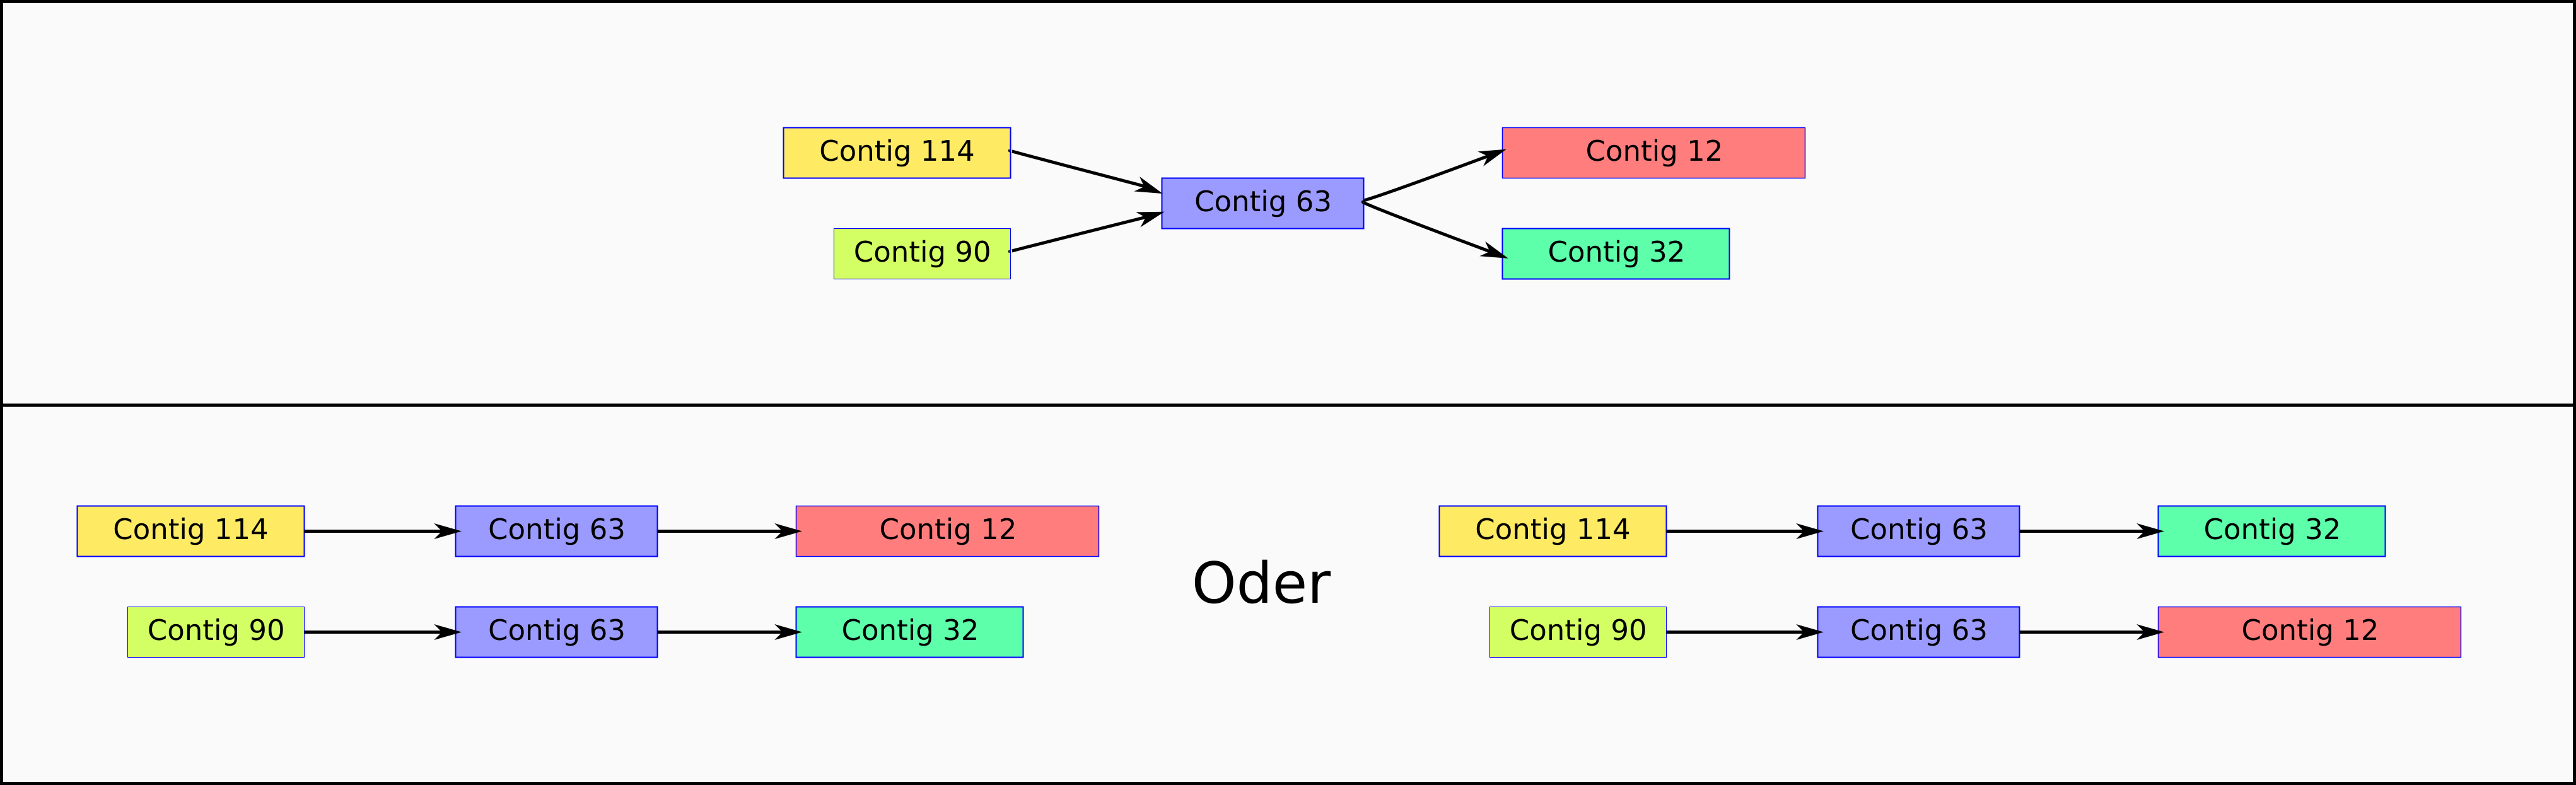
\includegraphics[width=0.9\textwidth]{bilder/repeat}
\end{center}
\caption{Repeat in einer Sequenz}
\label{repeat}
\end{figure}



Noch größere Schwierigkeiten machen eine andere Form von repetitiven Regionen in der DNA, bei denen sich zwei Regionen gleichen, welche 
%A19: sich eingefügt
sich in unterschiedlichen Bereichen in dem Strang befinden. Das Problem dieser Repeats wird in Abbildung \ref{repeat} verdeutlicht. 
%Noch größere Schwierigkeiten machen Regionen in der DNA, die über eine längere Strecke komplett identisch sind, sogenannte Repeats. Das Problem wird in Abbilding \ref{repeat} verdeutlicht. 
Zu sehen sind fünf Contigs, wobei ein Pfeil von Contig $a$ zu Contig $b$ bedeutet, dass in der DNA Contig $a$ direkt vor Contig $b$ kommt. Da Contig 63 (blau) zwei mal in der DNA vorkommt, ist es nicht trivial zu bestimmen, wie der Strang verläuft. 
% A19: Und 
Ferner ist MHC sehr repetitiv, somit werden viele Contigs mehrfach in der Sequenz auftauchen. Daher reichen die Daten aus Illumina nicht aus
%A19: Komma 
, um MHC zu assemblieren.


Eine weitere Möglichkeit der Sequenzierung ist die 
% A19: emph ergänzt 
\emph{Nanopore-Sequenzierung} \cite{Nanopore}. Hierbei können sehr lange Reads von 10\,000 bis über 1\,000\,000 Basenpaaren gelesen werden. Aufgrund des Längenunterschieds werden die Reads aus der 
% A19: Illuminar Sequenzierung 
Illumina-Sequenzierung auch \emph{Short-Reads} genannt 
% A19: ,
und die Reads aus der Nanopore-Sequenzierung \emph{Long-Reads}. Durch ihre Länge umfassen die Long-Reads oftmals bereits vollständige Repeats plus Umgebung. In 
Abbildung \ref{repeat} entspräche dies einem Read, in dem Contig 114, Contig 63 und Contig 32 (gelb, blau und grün) Teil von einem Read sind und es keine Schwierigkeiten diesbezüglich gibt. Leider ist die Fehlerrate bei dieser Methode sehr hoch \cite{Harris475194}. 
So werden sehr viele Long-Reads aus der selben Region benötigt, um die richtigen Basenpaare einigermaßen verlässlich zu bestimmen.


Daher hat die Manchot-Forschungsgruppe vom Institut für Medizinische Mikrobiologie und Krankenhaushygiene der HHU, mit deren Zusammenarbeit diese Arbeit entstand, eine Kombination der beiden Methoden entwickelt.
Die verlässlichen Contigs aus der 
Illumina-Sequenzierung wurden auf die Long-Reads gemappt und so deren Abstände zueinander bestimmt. 
Wir betrachten zur Anschauung Abbildung \ref{longread} eines Long-Reads. Die bunten Bereiche stellen Gebiete dar, in denen die Basenpaarsequenzen mit denen eines Contigs aus den 
Illumina-Daten übereinstimmen. In der selben Situation wie in Abbildung \ref{repeat} hätten wir nun die Information erhalten, dass Contig 114 und Contig 32 zusammengehören, also die rechte Auflösung der Abbildung richtig ist. 
\begin{figure}[b!]
\begin{center}

\includegraphics[width=0.8\textwidth]{bilder/longread}
\end{center}
\caption{Ein Long-Read über mehrere Contigs}
\label{longread}
\end{figure}
% A19: Absatz machen

Die Manchot-Forschungsgruppe hat diese Daten gesammelt und daraus eine Liste aus paarweisen Daten extrahiert. Diese besitzt die Form: Contig $a$ hat zu Contig $b$ die Entfernung $d$ (in Anzahl von Basenpaaren zwischen $a$ und $b$). Dieses Dreiertuple aus zwei Contigs und einer Distanz nennen wir einen \emph{Constraint}.


Es bleiben noch einige Schwierigkeiten für die Assemblierung zu beachten. Die Distanzwerte zwischen den Contigs sind meistens durch Fehler in den Long-Reads verfälscht. Dadurch sind erst mehrere Constraints, die eine ähnliche Distanz zwischen zwei Contigs prognostizieren, wirklich belastend. Bis zu 
% A19: welchen 
welcher Distanz sich Constraints noch bestätigen und ab wann sie sich widersprechen ist hierbei ein entscheidender Aspekt, der betrachtet werden muss. Die Repeats lassen sich nicht immer so eindeutig auflösen wie in unserem Beispiel. In manchen Fällen kann erst im Gesamtzusammenhang erkannt werden, wie der Strang verläuft. Letztlich bleibt noch die große Datenfülle als Herausforderung zu nennen: Bei rund 122\,000 auftretenden Distanzen zwischen 2\,124 Contigs ist eine manuelle Zusammenfügung nicht zielführend und mindestens eine Teilautomatisierung der Prozesse obligatorisch. Auf der anderen Seite sind die Constraints nicht gleichmäßg verteilt, sodass es Regionen gibt, bei denen mit sehr wenig Informationen ausgekommen werden muss.

Hier stellt sich die Frage, mit welchen Methoden diese Probleme bewältigt werden können. Denkbar wäre eine Umsetzung mittels 
\emph{Linearer Programmierung}. Das Ziel dieser Arbeit wird sein, zu untersuchen, ob lineare Programmierung hierbei anwendbar ist
 und welche Vor- und Nachteile lineare Programme mit sich bringen.
